\chapter{Proposed Methods}
% do i need this
In this chapter, we introduce the proposed methods and experimental methodology. This research aims to address the question, "What would happen if we change the masking strategies?" While numerous strategies have been proposed to enhance the representation of text and images, there has been limited experimentation on altering the masking ratio in masked language modeling (MLM). This study primarily focuses on two main aspects:

\begin{itemize}
  \item The referenced model employs masked language modeling to train feature extraction, maintaining a constant masking ratio throughout the training process. This research proposes varying the masking ratio and introducing a time-variant component during training.
  \item The referenced model includes a function known as momentum-based replace token detection, which also operates with a specific masking ratio. This study examines whether adjusting the masking ratio for this task, similar to the approach taken with MLM, improves prediction performance when both parameters are modified.
\end{itemize}
%%%
% \color{WIP}
The purpose of this experiment is to examine the hypothesis that time variant masking ratio affect the prediction on text based person retrieval.
This is carried out by investigating the relation and sensitivity aware representation learning \cite{Bai2023RaSaRA} that investigated the better representation learning for image and text inputs by detecting the replaced tokens from the converted text and corresponding image inputs. The results showed significant improvements in prediction performance. To investigate further towards the masking ratio, \cite{wettig-etal-2023-mask} investigated that larger models should adopt a higher masking rate rather than masking 15\% of tokens conventionally. Another method from Dongjie Yang, et al, \cite{yang2023learningbettermaskingbetter} proposed time-variant masking ratio decay strategy and POS-tagging weighed masking. In results, the time variant masking decay method outperformed the time invariant masking ratio for F1 score on SQuAD performance during pre-training on BERT-large model. 

In this experiment, we investigate the effect of the performance towards the time variant masking ratio on replaced token detection task. To evaluate the performance, we will compute the feature similarity score for all image-text pairs. Then we take top-$k$ candidates and calculate their ITM score $s_{itm}$ for ranking. 

\section{Dataset}

\begin{figure}[htbp]
  \begin{center}
      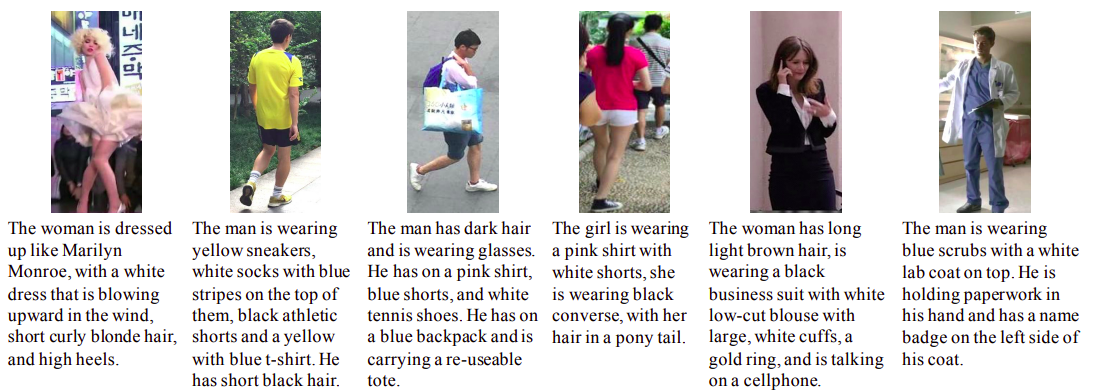
\includegraphics[width=\linewidth]{img/cuhk_pedes.png}
      \caption{Example sentence with corresponding image}
      \label{fig:cuhk_pedes}
  \end{center}
\end{figure}


Dataset we are using is CUHK-PEDES \cite{li2017personsearchnaturallanguage}. This is a large-scale dataset created to facilitate person search using natural language descriptions. It addresses the need for a dataset where persons are described in detail using natural language, enabling practical applications such as video surveillance. Key features of the dataset are shown as follows:
\begin{itemize}
  \item Large-scale: Dataset contains 40,206 images over 13,003 persons 
  \item Annotations: Each images is described with two sentences by independent annotators, in total of 80,412 sentence descriptions
  \item Source diversity: Images are sourced from a variety of existing person re-identification datasets, including CUHK03\cite{li2014deepreid}, Market-1501\cite{7410490}, SSM\cite{ssm}, VIPeR\cite{viper}, and CUHK01\cite{li2012human}.
\end{itemize}

The datasets contains image and corresponding natural language description as shown in Fig\ref{fig:cuhk_pedes}. Image source for CUHK-PEDES are from CUHK03, Market-1501, SSM, VIPER, and CUHK01. The annotations for each image are done by Amazon Mechanical Turk(AMT), which is a crowd workers that are employed to describe each image with two sentence. Each sentence include rich descriptions about person appearance, action poses, and interactions.


\section{Methods}
In this section, the experiment method will be introduced for the effect of performance with vision language models(VLM). VLM with recent SOTA models (\cite{Bai2023RaSaRA}) uses attention mechanism to extract both image and text features, and then both features are aligned with cross modality encoders. To achieve better results, feature extraction is important but also learning better textual representation is required to guide the interpretation of visual data. Thus, our aim is to train the visual language model with textual information representation with different strategies. We will experiment on two different methods to see the affect to the result.


\section{Masking ratio for mlm} 
To investigate the impact of varying the masking ratio on the performance of masked language models (MLMs). The study aims to determine the optimal masking ratio that balances training efficiency and model accuracy. 


Recently, textual information representation is done by masked language model 
For relation and sensitivity aware learning, they train the model with two tasks: relation aware and sensitivity aware. Relation aware distinguishes between strong and weak positive pairs in the dataset which allows to learn more effectively from the data. 
Sensitivity aware aims to make the model sensitive to specific transformations in the data, particularly textual changes. While many models aim to learn invariant representations that are robust to various data augmentations, RaSa takes it further by encouraging the model to detect and respond to sensitive transformations, such as word replacements in text. This is done using a Momentum-based Replaced Token Detection (M-RTD) task, where the model learns to detect whether a token in the text has been replaced. This sensitivity to changes enhances the robustness and discrimination power of the representations learned by the model.


\section{masking ratio for replaced token detection}
explanation about masking ratio changes on m-RTD





Predicting more means the model learns from more training signals, so higher prediction rates boost the model performance. From another perspective, each prediction at each masked token leads to a loss gradient, which is averaged to optimize the weights of the model. Averaging across more predictions has a similar effect to increasing the batch size, which is proved to be beneficial for pre-training (Liu et al., 2019). 


corruption rate how much we mask the words from the text
prediction rate how much we predict the mask token 


what i did 
- change the mask 
- visualize the attention section

The structure of the algorithm is done as follows. 
- image encoder
  mlp 
- text encoder
  bert 

When we work on fine tuning, we change the masking ratio on the mlm process. 
the masking ratio will be changed as follows.
flat 
cosine curve 
random 

from these papers, bert scored higher accuracies when using 40\% on masking ratio. This is basically done in text information, 
so we would like to try it out in text based image retireval tasks. T

flat and cosine will work on the range of 40\% and 60\% 
the previous work has been done as 15\%, so we would compare the results with that for the discussion 

\section{Requirements specification}

- model
rasa

- dataset 
CUHK-dataset
ICFG-dataset

- epoch
30

- learning rate 
1e-5 to 1e-6

\section{Attention visualization}
To be able to see where the model is paying attention to, we would use the attention matrix in cross atttention module.



\section{Algorithm implementation}

for the 